\documentclass[12pt,a4paper,UTF8]{article}
\usepackage{ctex}
\usepackage{amsmath,amscd,amsbsy,amssymb,latexsym,url,bm,amsthm}
\usepackage{epsfig,graphicx,subfigure}
\usepackage{balance}
\usepackage{enumerate}
\usepackage{wrapfig}
\usepackage{mathrsfs, euscript}
\usepackage[usenames]{xcolor}
\usepackage[CJKbookmarks, colorlinks, bookmarksnumbered=true,pdfstartview=FitH,linkcolor=black,citecolor=black]{hyperref}
\usepackage[vlined,ruled,commentsnumbered,linesnumbered]{algorithm2e}

\usepackage{fontspec}


\definecolor{bashback}{rgb}{0.2,0.1,0.1}
\definecolor{dkgreen}{rgb}{0,0.6,0}
\definecolor{gray}{rgb}{0.5,0.5,0.5}
\definecolor{mauve}{rgb}{0.58,0,0.82}

\newfontfamily\consolas{Consolas}
\newfontfamily\freesans{FreeSans}
\newfontfamily\cn{Courier New}
\newfontfamily\namefont{文泉驿等宽微米黑}
\newfontfamily\bashfont{Ubuntu Mono}
\newcommand{\mytitle}{\fontsize{15pt}{}\freesans\textbf}


\newtheorem{theorem}{Theorem}[section]
\newtheorem{lemma}[theorem]{Lemma}
\newtheorem{proposition}[theorem]{Proposition}
\newtheorem{corollary}[theorem]{Corollary}
\newtheorem{exercise}{Exercise}[section]
\theoremstyle{definition}


\numberwithin{equation}{section}
\numberwithin{figure}{section}

\renewcommand{\thefootnote}{\fnsymbol{footnote}}

\newcommand{\postscript}[2]
 {\setlength{\epsfxsize}{#2\hsize}
  \centerline{\epsfbox{#1}}}

\renewcommand{\baselinestretch}{1.0}

\setlength{\oddsidemargin}{-0.365in}
\setlength{\evensidemargin}{-0.365in}
\setlength{\topmargin}{-0.3in}
\setlength{\headheight}{0in}
\setlength{\headsep}{0in}
\setlength{\textheight}{10.1in}
\setlength{\textwidth}{7in}
\makeatletter
\usepackage{listings}
\usepackage{silence}
\WarningsOff*
\lstdefinestyle{cmdmod}
{
  language=bash,
  %xleftmargin=0.5cm,
  basicstyle=\footnotesize\bashfont\color{cyan},
	%numbers=left,                   % where to put the line-numbers
	numberstyle=\footnotesize\color{gray},  % the style that is used for the line-numbers
    backgroundcolor=\color{bashback},      % choose the background color. You must add \usepackage{color}
  %commentstyle=\color{red},
  %keywordstyle=\color{black},
  numberstyle=\tiny\cn \color{blue},
  %basicstyle=\small\cn
	showspaces=false,               % show spaces adding particular underscores
	showstringspaces=false,         % underline spaces within strings
	showtabs=false,                 % show tabs within strings adding particular underscores
	frame=single                   % adds a frame around the code
}
\lstdefinestyle{cmod}
{ %
	language=C,                % the language of the code
	xleftmargin=0.5cm,
	basicstyle=\footnotesize\consolas,       % the size of the fonts that are used for the code
	numbers=left,                   % where to put the line-numbers
	numberstyle=\footnotesize\color{gray},  % the style that is used for the line-numbers
	stepnumber=1,                   % the step between two line-numbers. If it's 1, each line 
	% will be numbered
	numbersep=5pt,                  % how far the line-numbers are from the code
	backgroundcolor=\color{white},      % choose the background color. You must add \usepackage{color}
	showspaces=false,               % show spaces adding particular underscores
	showstringspaces=false,         % underline spaces within strings
	showtabs=false,                 % show tabs within strings adding particular underscores
	frame=shadowbox,                   % adds a frame around the code
	rulecolor=\color{black},        % if not set, the frame-color may be changed on line-breaks within not-black text (e.g. commens (green here))
	tabsize=4,                      % sets default tabsize to 4 spaces
	captionpos=b,                   % sets the caption-position to bottom
	breaklines=true,                % sets automatic line breaking
	breakatwhitespace=false,        % sets if automatic breaks should only happen at whitespace
	%title=\lstname,                   % show the filename of files included with \lstinputlisting;
	% also try caption instead of title
	keywordstyle=\color{blue},          % keyword style
	commentstyle=\color{dkgreen},       % comment style
	stringstyle=\color{mauve},         % string literal style
	escapeinside={\%*}{*)},            % if you want to add LaTeX within your code
	morekeywords={*,...}               % if you want to add more keywords to the set
}

\newenvironment{solution}
{\par\vspace{3mm}\noindent{\textbf{Solution.}}}{\qed}
\renewcommand\contentsname{Contents}


\begin{document}
\title{\vspace{-0.5cm}\mytitle{CS356} \hspace{2cm}\mytitle{Operating System Projects} \hspace{2cm}\mytitle{Spring 2017}\\\vspace{0.5cm}\mytitle{Project 2: Android Memory Management}}
\author{
  yelantingfeng 
    }
\date{June 9, 2017}
\maketitle
\tableofcontents

\newpage

\section{Objectives}
\begin{enumerate}[ I]
    \item Compile the Android kernel.
    \item Familiarize Android page replacement algorithm.
    \item Get the target process's virtual address and physical address.
    \item Implement a counting algorithm page replacement.
  \end{enumerate}

\section{Project Environment}
\textbf{Implementation:} AVD(Android Virtual Devices), SDK version r24.4.1

\textbf{Linux (64-bits):} Ubuntu 16.04 LTS

\begin{center}

\includegraphics[scale=0.3]{Android.png}\\

\includegraphics[scale=0.14]{ubuntu.jpg}
\end{center}

\newpage
\section{Details for Implementation}
\subsection{Problem \uppercase\expandafter{\romannumeral1} : Compile the kernel}
\subsubsection{Description}
Our task for this problem is to learn how to change the configs of the compilation of the kernel by modifying Makefile and using ncurses-dev. This is the basis of the tasks behind.
\subsubsection{Analysis}
This problem is the easiest part of the whole project. We just need to follow the following steps and then we can make everything right.

\begin{enumerate}[a.]
  \item Make sure that you have added the following path into your environment variable.
    \begin{lstlisting}[style=cmdmod]
ANDROID_NDK_HOME/toolchains/arm-linux-androideabi-4.6/prebuilt/linux-x86_64/bin
    \end{lstlisting}
    To achieve this, you can append some codes in {\color{blue}$\thicksim$/.bashrc}, a hidden file in you home directory.
  \item Open {\color{blue}Makefile} in {\color{blue}KERNEL\_SOURCE/goldfish/} and find these:
    \begin{lstlisting}[style=cmdmod]
    ARCH       ?= $(SUBARCH)
    CROSS_COMPILE ?=
    \end{lstlisting}
    Change it to:
    \begin{lstlisting}[style=cmdmod]
    ARCH       ?= arm
    CROSS_COMPILE ?= arm-linux-androideabi-
    \end{lstlisting}
    Save it and exit.
  \item Execute the following command in terminal to set compiling config:
    \begin{lstlisting}[style=cmdmod]
$ make goldfish_armv7_defconfig
    \end{lstlisting}
    \item Modify compiling config:
      \begin{lstlisting}[style=cmdmod]
$ sudo apt-get install ncurses-dev
$ make menuconfig
    \end{lstlisting}
    Then you can see a GUI config. Open the {\bashfont\color{cyan} Compile the kernel with debug info} in {\bashfont\color{cyan} Kernel hacking} and {\bashfont\color{cyan} Enable loadable module support} with {\bashfont\color{cyan} Forced module loading}, {\bashfont\color{cyan} Module unloading} and {\bashfont\color{cyan} Forced module unloading} in it. Save it and exit.
    \item Compile.
      \begin{lstlisting}[style=cmdmod]
$ make -j4
    \end{lstlisting}
    The number of {\bashfont\color{cyan}-j*} depends on the number of cores of your CPU.
\end{enumerate}


\subsection{Problem \uppercase\expandafter{\romannumeral2} : Map a target process's Page Table}
\subsubsection{Description}
In the Linux kernel, the page table is broken into multiple levels. For ARM64-based devices, a three-level paging mechanism is used. For this problem, we are going to implement the following two system call interfaces, and then use them to implement an VATranslate program to test our calls, which can get the physical address via command {\color{cyan}\bashfont./VATranslate \#pid \#VA} . The required system call interfaces are as follows. 

\begin{lstlisting}[style=cmod]
struct pagetable_layout_info {
  uint32_t pgdir_shift;
  uint32_t pmd_shift;
  uint32_t page_shift;
};

int get_pagetable_layout(struct pagetable_layout_info __user * pgtbl_info, int size);
\end{lstlisting}
\begin{lstlisting}[style=cmod]
int expose_page_table(pid_t pid,unsigned long fake_pgd,unsigned long fake_pmds,unsigned long page_table_addr,unsigned long begin_vaddr,unsigned long end_vaddr);
\end{lstlisting}
\subsubsection{Analysis}
I think it is a better way to add system calls by writing a module. The reason is that once you have already booted your virtual device, if you want to make some change on your system call, you do not need to reboot your device. This is important to shorten our debug process.

The first system call is not too difficult. I firstly searched PGD\_SHIFT on \href{http://elixir.free-electrons.com/linux/v3.4.67/ident/}{linux-Elixir-Free Electrons}, and I note that we should select the kernel version v3.4.67. Then I found it defined in some {\color{blue}arch/arm/include/asm/pgtable*.h}. Since we've already included {\color{blue}include/linux/sched.h}, which includes {\color{blue}pgtable.h}, so all that we need to do is just to copy these given macros to user space. You can see some more details in the first code of Solution part.

To finish the second system call, I have done a lot of homework. Before I start to implement this call, I wrote a small application to test the first call and then found that it is using 2-level paging mechanism. To finish this task, I involked three functions in kernel, {\color{cyan}\bashfont find\_get\_pid}, {\color{cyan}\bashfont walk\_page\_range} and {\color{cyan}\bashfont remap\_pfn\_range}, but the second function has not been exported for module programming. To invoke it in our module, we have to modify two files in the kernel. We add {\color{cyan}\bashfont extern} before the function prototype of {\color{cyan}\bashfont walk\_page\_range} in {\color{blue}include/linux/mm.h}. And then add two lines below in {\color{blue} mm/pagewalk.c}.
\begin{lstlisting}[style=cmod]
#include <linux/export.h>
EXPORT_SYMBOL(walk_page_range);
\end{lstlisting}
The function {\color{cyan}\bashfont walk\_page\_range} can recursively walk the page table for the memory area in VMA. And {\color{cyan}\bashfont remap\_pfn\_range} can remap the given physical frame to userspace. You can see some more details in the second code of Solution part.

Once we have finished these two system calls, it is easy to implement an VATranslate program. We just need to use the first one to get the layout and the second one to copy necessary page table to our memory space. Then we can use the page table and the fake page directory to translate the virtual address. Note that the lower 12 bits of each entry are used to store some information, so we should mask them when do the translation. For more details, you can read the third code in Solution part.
\subsubsection{Solution}
{\color{red}I just show the critical part of my solution code.}
\lstinputlisting[style=cmod]{layout.c}
\lstinputlisting[style=cmod]{expose.c}
\newpage
\lstinputlisting[style=cmod]{VATranslate.c}

\subsubsection{Output}
Firstly, we should install our mod.
\begin{lstlisting}[style=cmdmod]
$ cd /data/misc
$ insmod *.ko
\end{lstlisting}
Then we we can use {\color{cyan}\bashfont ./VATranslate \#pid \#VA} to do the translation. Note that not all the process have virtual memory information, to verify this, you can just easily use the command {\color{cyan}\bashfont cat} to check whether the {\color{blue} /proc/\#pid/maps} is empty. Here is a screenshot of my output.

\begin{center}
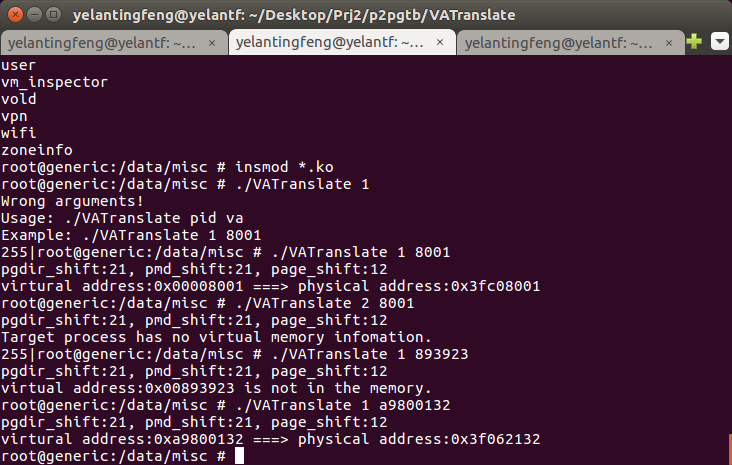
\includegraphics[scale=0.65]{vatranslate.png}
\end{center}
And some kern info may give me some more help.
\begin{center}
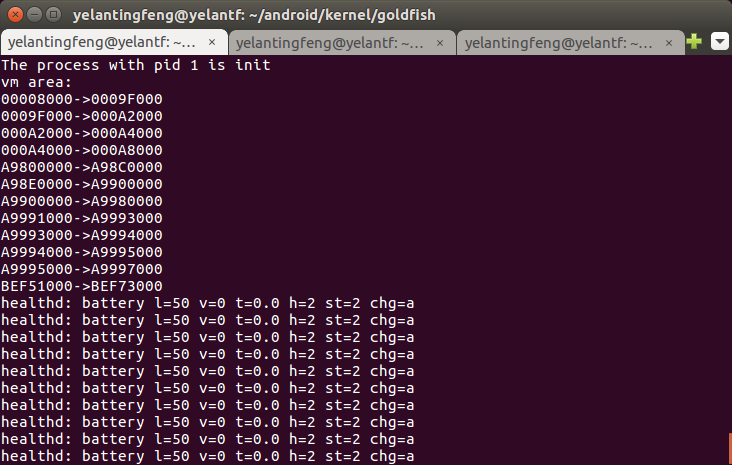
\includegraphics[scale=0.65]{vatranslate2.png}
\end{center}
\newpage

\subsection{Problem \uppercase\expandafter{\romannumeral3} : Investigate Android Process Address Space}
\subsubsection{Description}
Implement a program called {\color{cyan}\bashfont vm\_inspector} to dump the page table entries of a process in given range. To dump the PTEs of a target process, you will have to specify a process identifier "pid" to {\color{cyan}\bashfont vm\_inspector}. Use this program to investigate some process' address space, including Zygote. Refer to {\color{blue} /proc/pid/maps} in your AVD to get the memory maps of a target process and use it as a
reference to find the different and the common parts of page table dumps between Zygote
and an Android app.
\subsubsection{Analysis}
After finishing problem 2, this problem is easy. We just need to round the start virtual address and end virtual address to page start and page end and allocate enough space for our page table and fake pgd. Then we just happily print the entries in the page table from given start virtual address to given end virtual address.
\subsubsection{Solution}
\lstinputlisting[style=cmod]{vm_inspector.c}
\subsubsection{Output}
Still, install the module first and then we can use {\color{cyan}\bashfont vm\_inspector \#pid \#begin\_vaddr \#end\_vaddr} to dump the page tables of target process. Once you start an App, you can use command {\color{cyan}\bashfont ps} to see the pid of the App and you can easily find that page table changes as you play with this App.

Then I dump the page tables of Zygote and Calculator and reference the maps file of them simultaneously. We can easily found that they share so many things in their memory. Then I googled this and found that Zygote is the parent process of most applications, so they share much in their memory. This memory are read-only and this design speed up the launch of applications. Here is a example screenshot of their shared objects.

\begin{center}
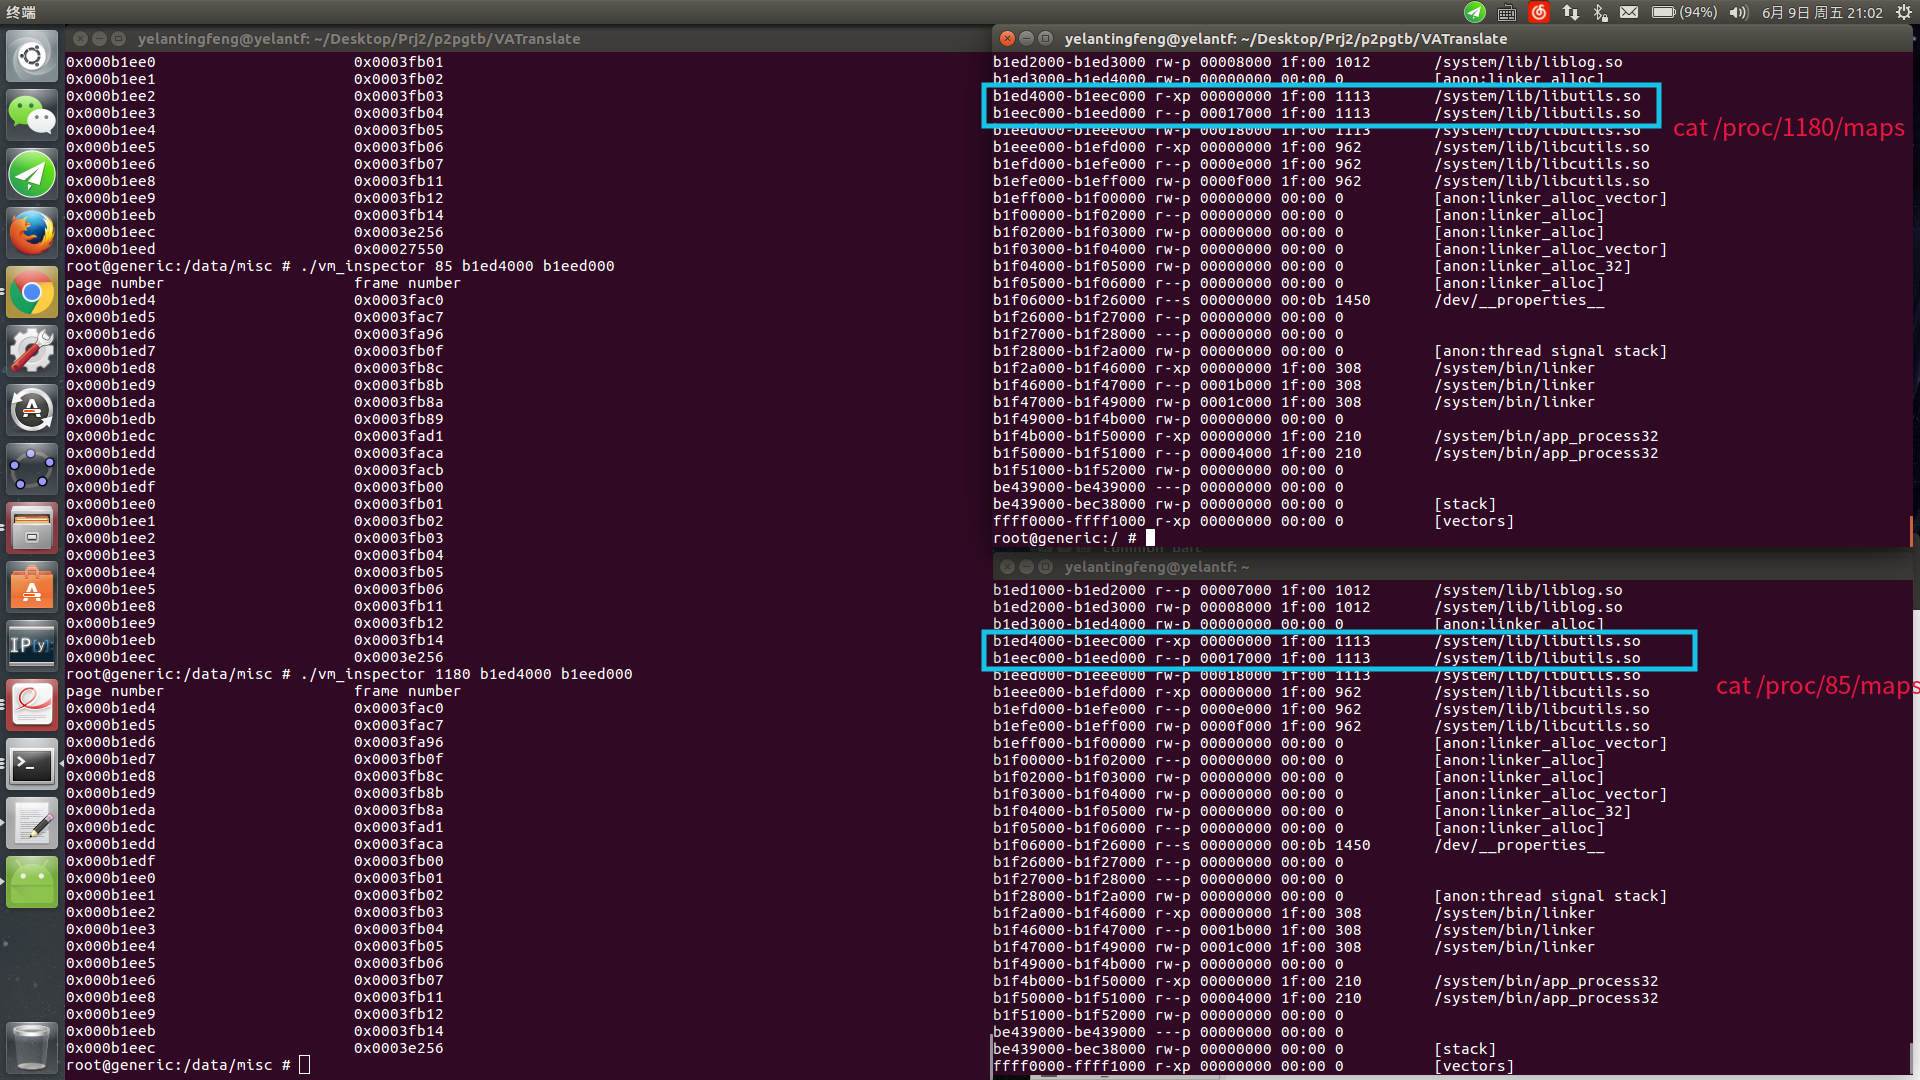
\includegraphics[scale=0.27]{zygotecommon.png}
\end{center}
\newpage

\subsection{Problem \uppercase\expandafter{\romannumeral4}: Change Linux Page Replacement Algorithm}
\subsubsection{Description}
The task for this problem is to change the page replacement algorithm. We should add a new reference variable to record the last time when this page was referenced. If a page is referenced by process, the referenced value of it should be set to 0. Otherwise, the
referenced value increases 1 for every period until it is referenced. We should check
these two lists periodically, move the page, whose reference vale is 0, to active list, and
move the page, whose referenced value larger than a threshold that defined by yourself,
to inactive list. To accomplish this algorithm, {\color{cyan}\bashfont kswapd()} and {\color{blue}/proc/meminfo} will be helpful.
\subsubsection{Analysis}
To change the page replacement algorithm, we need to know how the page replacement algorithm works in detail. I think this \href{http://blog.csdn.net/zouxiaoting/article/details/8824896}{article} helps a lot. The key part of our task is to add a variable in page struct in {\color{blue}include/linux/mm\_types.h} and do some modification on some functions in {\color{blue}mm/vmscan.c} and {\color{blue}mm/swap.c}.
\subsubsection{Solution}
{\color{red}I just show the critical part of my solution code.}
\begin{lstlisting}[style=cmod]
//include/linux/mm_types.h
struct page{
    //------
    //------
    /* Our added variable.*/
    unsigned long lastRefTime;
};
\end{lstlisting}
\begin{lstlisting}[style=cmod]
//mm/vmscan.c
//------
#define MY_TIME_THRES 2

static void shrink_active_list(unsigned long nr_to_scan,
                                struct mem_cgroup_zone *mz,
                                struct scan_control *sc,
                                int priority, int file)
{
  //------
    if (page_referenced(page, 0, mz->mem_cgroup, &vm_flags)) {
        //let our variable be zero.
        printk(KERN_INFO"%ld:Found page referenced in shrink_active_list. variable set to 0.\n",page->index);
        page->lastRefTime=0;
        //---------
    }
    else if\left( ++page->lastRefTime) <= MY_TIME_THRES ){
        printk(KERN_INFO"%ld:Found page not refereced in shrink_active_list, variable=%u, not exceeded yet.\n",page->index,page->lastRefTime);
        list_add(&page->lru, &l_active);
        continue;
    }

    printk(KERN_INFO"%ld:Found page not refereced in shrink_active_list, variable=%u, shrinked.\n",page->index,page->lastRefTime);\right);
    //--------
}

//---------

static enum page_references page_check_references(struct page *page,
                          struct mem_cgroup_zone *mz,
                          struct scan_control *sc)
{
  //-------
  if (referenced_ptes) {
            printk(KERN_INFO"%ld:Found referenced in shrink_inactive_list, activate page referenced with variable=0.\n",page->index);
            page->lastRefTime=0;
            return PAGEREF_ACTIVATE;
            //-----------
          }
    //-------
}
\end{lstlisting}
\begin{lstlisting}[style=cmod]
//mm/swap.c
//---------
void mark_page_accessed(struct page *page)
{
    page->lastRefTime=0;
    if (!PageActive(page) && !PageUnevictable(page) &&
                PageLRU(page)) {
        activate_page(page);
    }
}
\end{lstlisting}
\newpage
\subsubsection{Output}
After I write a program to occupy a lot of memory, I get kernel info like this,
\begin{center}
  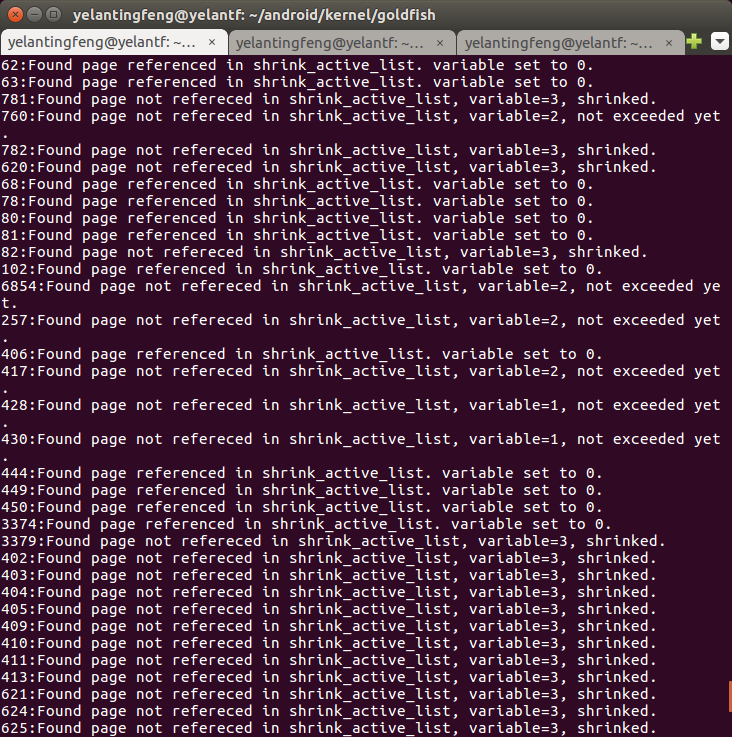
\includegraphics[scale=0.7]{pgreplace.png}
\end{center}
this implies my algorithm works. If we set the threshold to a very high value, like 20, the system will crash since there memory is so tense. And after I change the algorithm and set a proper threshold, everything keeps stable and okay, so it is reasonable to say that I change the algorithm successfully.
\newpage

\section{Discussion}
    After finish this project, I have a much more deep insight with linux memory management. I know much more about the kernel space and user space, which is exactly what keeps a operating system safe from unsafe operating. The amout of coding of this project is not so much, but we have to read much more than code. By reading the code of our kernel Implementation and the article about kernel memory management, we know more clearly about their actual structure and I think it a precious gift from this project. I am grateful to my classmates who discuss with me and TAs who provide me so much help. Thanks a lot!
\end{document}
